\documentclass[tikz]{standalone}
\usepackage{amsmath}
\definecolor{bgdark}{HTML}{171D2B}
\definecolor{aksen}{HTML}{F7B538}
\definecolor{batang}{HTML}{3B4A6B}
\begin{document}
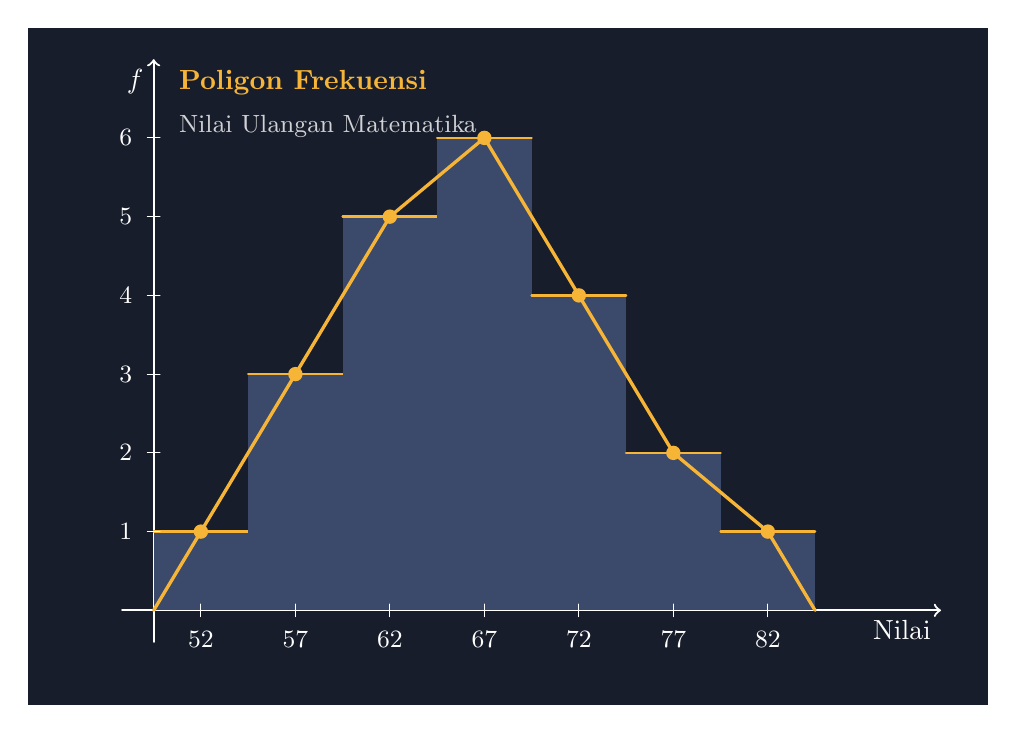
\begin{tikzpicture}[line cap=round, line join=round]
\fill[bgdark] (-1.6,-1.2) rectangle (10.6,7.4);
% sumbu
\draw[white, thick, ->] (-0.4,0) -- (10.0,0) node[below left, text=white] {Nilai};
\draw[white, thick, ->] (0,-0.4) -- (0,7.0) node[below left, text=white] {$f$};
% titik tengah kelas dan frekuensi
% kelas: 50-54(1),55-59(3),60-64(5),65-69(6),70-74(4),75-79(2),80-84(1)
% tengah: 52,57,62,67,72,77,82 -> skala x: x = (t-52)*1.2
\def\dx{1.2}
\foreach \t/\f/\lab in {52/1/1,57/3/3,62/5/5,67/6/6,72/4/4,77/2/2,82/1/1}{
  \pgfmathsetmacro\xx{0.6+(\t-52)/5*1.2}
  \fill[batang] (\xx-0.6,0) rectangle (\xx+0.6,\f);
  \draw[aksen, line width=0.9pt] (\xx-0.6,\f) -- (\xx+0.6,\f);
}
% poligon: titik tengah puncak batang + ujung tertutup di garis sumbu
\pgfmathsetmacro\xA{0}
\def\xB{8.4}
\draw[aksen, very thick]
  (\xA,0) -- (0.6,1) -- (1.8,3) -- (3.0,5) -- (4.2,6) -- (5.4,4) -- (6.6,2) -- (7.8,1) -- (\xB,0);
\foreach \px/\py in {0.6/1,1.8/3,3.0/5,4.2/6,5.4/4,6.6/2,7.8/1}{
  \fill[aksen] (\px,\py) circle (2.6pt);
}
% label frekuensi di sumbu y
\foreach \fy in {1,2,3,4,5,6}{
  \draw[white] (-0.08,\fy) -- (0.08,\fy);
  \node[left, text=white, font=\small] at (-0.15,\fy) {\fy};
}
% label titik tengah kelas di sumbu x
\foreach \t in {52,57,62,67,72,77,82}{
  \pgfmathsetmacro\xx{0.6+(\t-52)/5*1.2}
  \draw[white] (\xx,-0.08) -- (\xx,0.08);
  \node[below, text=white, font=\small] at (\xx,-0.15) {\t};
}
% keterangan
\node[text=aksen, font=\bfseries, anchor=west] at (0.2,6.7) {Poligon Frekuensi};
\node[text=white!80!bgdark, font=\small, anchor=west] at (0.2,6.15) {Nilai Ulangan Matematika};
\end{tikzpicture}
\end{document}
